\documentclass[aspectratio=169]{beamer}
\usepackage{amsmath}
\usepackage{amssymb}
\usepackage{tikz}
\usepackage{wasysym}
\usepackage{tikzsymbols}
\usepackage{xcolor}
\usepackage{animate}     % Option 1: play a PNG frame sequence
\usepackage{multimedia}  % Option 2: embed a video file (needs -shell-escape)
\usetikzlibrary{shapes,backgrounds,patterns}

% --- added for these slides -------------------------------------------------
\usepackage{pgfplots}
\pgfplotsset{compat=1.18, legend cell align=left}
\usetikzlibrary{arrows.meta,decorations.pathreplacing,calc,positioning}
\usepackage{listings}
\usepackage{booktabs}
% ----------------------------------------------------------------------------

% royalblue isn't a base xcolor name, so define it first (this is the default accent)
\definecolor{royalblue}{RGB}{65,105,225}

% ============================================================
%  ACCENT COLOR: change ONE line below to switch the theme
%  Choose one of: royalblue , red , black
% ============================================================
\colorlet{accent}{royalblue}
% \colorlet{accent}{red}
% \colorlet{accent}{black}
% ============================================================

% Use default theme with white background
\usetheme{default}

% Make everything white/black, with the chosen accent color for structure
\setbeamercolor{background canvas}{bg=white}
\setbeamercolor{normal text}{fg=black}
\setbeamercolor{structure}{fg=accent}
\setbeamercolor{frametitle}{fg=accent,bg=white}
\setbeamercolor{title}{fg=accent}
\setbeamercolor{section in toc}{fg=black}
\setbeamercolor{block title}{fg=black,bg=gray!10}
\setbeamercolor{block body}{fg=black,bg=gray!5}
\setbeamercolor{block title example}{fg=black,bg=green!10}
\setbeamercolor{block body example}{fg=black,bg=green!5}
\setbeamercolor{block title alerted}{fg=black,bg=red!10}
\setbeamercolor{block body alerted}{fg=black,bg=red!5}

\usepackage{scalerel}

\newcommand{\subsmall}[1]{_{\scaleto{#1}{4pt}}}
\newcommand{\supsmall}[1]{^{\scaleto{#1}{2pt}}}

% Remove navigation symbols
\setbeamertemplate{navigation symbols}{}

% Simple footline with page numbers (single definition)
\setbeamertemplate{footline}{
    \hfill\makebox[5pt]{%
        \scriptsize\insertframenumber}
    \hspace*{2em}
    \vspace{0.5cm}
}

% Custom command for colored boxes
\newcommand{\cbox}[2]{\colorbox{#1}{\ensuremath{\displaystyle #2}}}

% --- code listings (Python), coloured with the accent -----------------------
\lstdefinestyle{py}{
  language=Python,
  basicstyle=\ttfamily\footnotesize,
  keywordstyle=\color{accent}\bfseries,
  commentstyle=\color{gray}\itshape,
  stringstyle=\color{green!45!black},
  showstringspaces=false,
  columns=fullflexible,
  keepspaces=true,
  backgroundcolor=\color{gray!6},
  frame=single, rulecolor=\color{gray!30},
  xleftmargin=2pt, xrightmargin=2pt,
  escapeinside={(*}{*)}
}
\lstset{style=py}

% --- shared style for the small "what can go wrong" pictures -----------------
\pgfplotsset{
  miniplot/.style={
    width=4.0cm, height=3.0cm,
    axis lines=middle, xtick=\empty, ytick=\empty,
    samples=120, thick, clip=true
  }
}

\title{Root Finding II: Newton's Method}
\subtitle{Tangent lines and quadratic convergence}
\author{Sharareh Sayyad}
\institute{Washington State University}
\date{\today}

\begin{document}

% Title Slide
\frame{\titlepage}

% Table of Contents
\begin{frame}{Outline}
\tableofcontents
\end{frame}

% ============================================================
\section{From brackets to tangents}
% ============================================================

\begin{frame}{Recap: bracketing is reliable, but slow}
\begin{columns}[T]
\begin{column}{0.5\textwidth}
\small
Last lecture: bisection and false position.
\begin{itemize}
  \item \textbf{Always} converge once we have a bracket.
  \item Only \textbf{linear}: bisection gains one bit per step, $\approx 20$ steps for $10^{-6}$.
  \item Need a \textbf{sign change}: they cannot find the root of $(x-1)^2$.
\end{itemize}
\vspace{0.1cm}
\begin{block}{Today}
Use the \textbf{derivative} $f'(x)$ as well as $f(x)$. We give up the guarantee and get much more speed:
\[
\text{correct digits roughly \textbf{double} every step.}
\]
\end{block}
\end{column}
\begin{column}{0.46\textwidth}
\centering
\footnotesize
\setlength{\tabcolsep}{4pt}
\begin{tabular}{lc}
\toprule
$\sqrt2$, \ tol $= 10^{-6}$ & steps \\
\midrule
bisection on $[1,2]$ & 20 \\
false position on $[1,2]$ & 8 \\
Newton from $x_0 = 1$ & \cbox{green!15}{4} \\
\bottomrule
\end{tabular}

\vspace{0.4cm}
\begin{alertblock}{The trade-off}
\scriptsize Newton needs \textbf{no bracket}, only a starting guess $x_0$. But it can fail if $x_0$ is poor: it is a \textbf{local} method.
\end{alertblock}
\end{column}
\end{columns}
\end{frame}

\begin{frame}{The idea: follow the tangent line}
\begin{columns}[c]
\begin{column}{0.48\textwidth}
\small
Near $x_n$, replace $f$ by its \textbf{tangent line}:
\[
\ell(x) = f(x_n) + f'(x_n)\,(x - x_n).
\]
Take the zero of $\ell$ as the next guess:
\[
\cbox{accent!12}{x_{n+1} = x_n - \frac{f(x_n)}{f'(x_n)}}
\]
\vspace{0.05cm}
\begin{exampleblock}{Compare with false position}
False position: zero of a \textbf{secant} through two bracket points.\\
Newton: zero of the \textbf{tangent} at one point; no bracket is kept.
\end{exampleblock}
\end{column}
\begin{column}{0.5\textwidth}
\centering
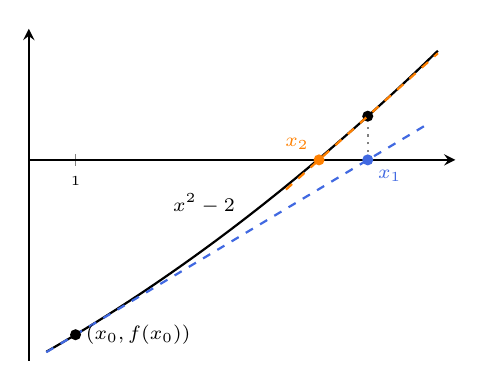
\begin{tikzpicture}
\begin{axis}[width=7cm, height=5.8cm, axis lines=middle, xmin=0.92, xmax=1.65, ymin=-1.15, ymax=0.75,
  xtick={1}, ytick=\empty, samples=80, thick, tick label style={font=\tiny}, clip=false]
  \addplot[black, domain=0.95:1.62] {x^2-2};
  \node[font=\scriptsize] at (axis cs:1.22,-0.25) {$x^2-2$};
  % tangent at x0 = 1
  \addplot[accent, dashed, domain=0.95:1.6] {-1+2*(x-1)};
  \fill (axis cs:1,-1) circle (2pt) node[right, font=\scriptsize] {$(x_0, f(x_0))$};
  % step to x1 = 1.5
  \draw[gray, dotted, thick] (axis cs:1.5,0) -- (axis cs:1.5,0.25);
  \fill (axis cs:1.5,0.25) circle (2pt);
  % tangent at x1 = 1.5
  \addplot[orange, dashed, domain=1.36:1.62] {0.25+3*(x-1.5)};
  \fill[accent] (axis cs:1.5,0) circle (2pt);
  \node[accent, font=\scriptsize, below right] at (axis cs:1.5,0) {$x_1$};
  \fill[orange] (axis cs:1.41667,0) circle (2pt);
  \node[orange, font=\scriptsize, above left] at (axis cs:1.41667,0) {$x_2$};
\end{axis}
\end{tikzpicture}\\[2pt]
\scriptsize $x_0 = 1 \;\to\; x_1 = 1.5 \;\to\; x_2 = 1.41\overline{6}$:\\ already within $0.0025$ of the root $\sqrt2$.
\end{column}
\end{columns}
\end{frame}

\begin{frame}{Where the formula comes from: Taylor's theorem}
\begin{columns}[T]
\begin{column}{0.54\textwidth}
\small
Expand $f$ around the current guess $x_n$:
\[
f(x) = f(x_n) + f'(x_n)(x - x_n) + \tfrac12 f''(\xi)(x - x_n)^2 .
\]
\begin{itemize}
  \item Drop the quadratic term: $f(x) \approx \ell(x)$, the tangent line.
  \item Solve $\ell(x) = 0$ for $x$: that is $x_{n+1}$.
\end{itemize}
\vspace{0.1cm}
\begin{block}{Newton = solve a linear model, repeat}
Each step replaces a hard problem (nonlinear $f$) by an easy one (a line). The neglected term is $O\big((x - x_n)^2\big)$, which is why the method is so fast once $x_n$ is close.
\end{block}
\end{column}
\begin{column}{0.42\textwidth}
\begin{alertblock}{Requirement}
\footnotesize We need a formula (or code) for $f'(x)$, and $f'(x_n) \neq 0$.
\end{alertblock}
\end{column}
\end{columns}
\end{frame}

% ============================================================
\section{Newton's method in practice}
% ============================================================

\begin{frame}[fragile]{Newton's method in Python}
\begin{columns}[T]
\begin{column}{0.56\textwidth}
\begin{lstlisting}[basicstyle=\ttfamily\scriptsize]
def newton(f, df, x0, tol=1e-10, maxit=50):
    x = x0
    for n in range(maxit):
        fx, dfx = f(x), df(x)  # two evaluations
        if dfx == 0:
            raise ZeroDivisionError("f'(x) = 0")
        dx = fx / dfx          # Newton step
        x = x - dx
        if abs(dx) < tol:      # step-size test
            return x
    raise RuntimeError("no convergence")
\end{lstlisting}
\end{column}
\begin{column}{0.41\textwidth}
\begin{alertblock}{Raise, don't return}
\footnotesize
Newton \textbf{may not converge}, so hitting \texttt{maxit} is an \textbf{error}, not a result. Never silently return the last $x$.
\end{alertblock}
\vspace{0.05cm}
\begin{block}{Cost per step}
\footnotesize
One $f$ \textbf{and} one $f'$ evaluation. If $f'$ is expensive or unknown, this matters (see Newton without derivatives).
\end{block}
\vspace{0.05cm}
\begin{block}{Why test the step $|dx|$?}
\scriptsize No bracket, no error bound, but the Newton step is an excellent error estimate (later).
\end{block}
\end{column}
\end{columns}
\end{frame}

\begin{frame}{Example: $\sqrt2$ by Newton, $f(x) = x^2 - 2$, $x_0 = 1$}
\begin{columns}[c]
\begin{column}{0.64\textwidth}
\centering
\footnotesize
\setlength{\tabcolsep}{3.5pt}
\begin{tabular}{rlcc}
\toprule
$n$ & \multicolumn{1}{c}{$x_n$} & $|x_n - \sqrt2|$ & $\dfrac{|e_n|}{|e_{n-1}|^2}$ \\
\midrule
0 & 1.0 & $4.1\times10^{-1}$ & \\
1 & 1.5 & $8.6\times10^{-2}$ & 0.500 \\
2 & \textbf{1.41}6666666666667 & $2.5\times10^{-3}$ & 0.333 \\
3 & \textbf{1.41421}5686274510 & $2.1\times10^{-6}$ & 0.353 \\
4 & \textbf{1.41421356237}4690 & $1.6\times10^{-12}$ & 0.354 \\
5 & \textbf{1.414213562373095} & $\le 2.2\times10^{-16}$ & \\
\bottomrule
\end{tabular}\\[4pt]
\scriptsize Bold digits are correct.
\end{column}
\begin{column}{0.33\textwidth}
\small
\begin{itemize}
  \item Correct digits: $2, 6, 12, 16$. They \textbf{double} each step until machine precision.
  \item The ratio $|e_n|/|e_{n-1}|^2$ settles to a constant:
  \[
  C = \frac{1}{2\sqrt2} \approx 0.354.
  \]
  \item Compare: bisection needs $\approx 52$ steps to reach full precision.
\end{itemize}
\end{column}
\end{columns}
\end{frame}

% ============================================================
\section{Quadratic convergence}
% ============================================================

\begin{frame}{Why the digits double}
\begin{columns}[T]
\begin{column}{0.53\textwidth}
\small
Let $e_n = x_n - r$. Taylor around $x_n$, evaluated at the root:
\[
0 = f(r) = f(x_n) - f'(x_n)\,e_n + \tfrac12 f''(\xi_n)\,e_n^2 .
\]
Divide by $f'(x_n)$ and use the Newton formula:
\[
\underbrace{x_n - \frac{f(x_n)}{f'(x_n)}}_{x_{n+1}} - r \;=\; \frac{f''(\xi_n)}{2f'(x_n)}\,e_n^2
\]
\[
\Longrightarrow\quad
\cbox{accent!12}{e_{n+1} \approx \frac{f''(r)}{2f'(r)}\,e_n^2}
\]
\end{column}
\begin{column}{0.44\textwidth}
\begin{block}{Order of convergence $p$}
\footnotesize $|e_{n+1}| \approx C\,|e_n|^{p}$.
\begin{itemize}
  \item $p = 1$: linear (bisection, false position)
  \item $p \approx 1.44$: Illinois
  \item $p = 2$: \textbf{quadratic} (Newton)
\end{itemize}
\end{block}
\scriptsize If $e_n \approx 10^{-k}$ then $e_{n+1} \approx C\cdot10^{-2k}$: twice as many digits.
\end{column}
\end{columns}
\end{frame}

\begin{frame}{The convergence theorem: fast, but only locally}
\begin{columns}[T]
\begin{column}{0.5\textwidth}
\begin{block}{Theorem (local convergence)}
\small Let $f$ be twice continuously differentiable near $r$, with $f(r) = 0$ and $f'(r) \neq 0$. Then there is a $\delta > 0$ such that for every $x_0$ with $|x_0 - r| < \delta$, Newton's method converges to $r$ \textbf{quadratically}.
\end{block}
\vspace{0.1cm}
\small
Read the fine print:
\begin{itemize}
  \item ``$x_0$ close enough'': the theorem does \textbf{not} say how close. $\delta$ can be tiny.
  \item ``$f'(r) \neq 0$'': a \textbf{simple} root. Double roots are slower.
\end{itemize}
\end{column}
\begin{column}{0.47\textwidth}
\centering
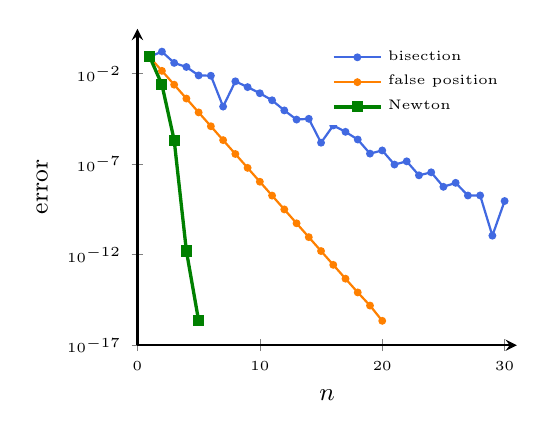
\begin{tikzpicture}
\begin{axis}[width=6.4cm, height=5.6cm, ymode=log, axis lines=left,
  xmin=0, xmax=31, ymin=1e-17, ymax=3, xlabel={$n$}, ylabel={error},
  thick, tick label style={font=\tiny}, label style={font=\small},
  legend style={font=\tiny, draw=none, at={(0.99,0.97)}, anchor=north east}]
  \addplot[accent, mark=*, mark size=1pt] coordinates {(1,0.0858) (2,0.164) (3,0.0392) (4,0.0233) (5,0.00796) (6,0.00766) (7,0.000151) (8,0.00376) (9,0.0018) (10,0.000826) (11,0.000337) (12,9.31e-05) (13,2.9e-05) (14,3.2e-05) (15,1.53e-06) (16,1.37e-05) (17,6.1e-06) (18,2.29e-06) (19,3.82e-07) (20,5.72e-07) (21,9.5e-08) (22,1.43e-07) (23,2.42e-08) (24,3.54e-08) (25,5.6e-09) (26,9.3e-09) (27,1.85e-09) (28,1.87e-09) (29,1.12e-11) (30,9.2e-10)};
  \addlegendentry{bisection}
  \addplot[orange, mark=*, mark size=1pt] coordinates {(1,0.0809) (2,0.0142) (3,0.00245) (4,0.00042) (5,7.21e-05) (6,1.24e-05) (7,2.12e-06) (8,3.64e-07) (9,6.25e-08) (10,1.07e-08) (11,1.84e-09) (12,3.16e-10) (13,5.42e-11) (14,9.3e-12) (15,1.59e-12) (16,2.74e-13) (17,4.71e-14) (18,8.22e-15) (19,1.55e-15) (20,2.22e-16)};
  \addlegendentry{false position}
  \addplot[green!50!black, mark=square*, mark size=1.4pt, very thick] coordinates {(1,0.0858) (2,0.00245) (3,2.12e-06) (4,1.59e-12) (5,2.22e-16)};
  \addlegendentry{Newton}
\end{axis}
\end{tikzpicture}\\[2pt]
\scriptsize $x^2-2$. Linear methods give straight lines on \texttt{semilogy}; Newton's curve \textbf{bends down}: quadratic.
\end{column}
\end{columns}
\end{frame}

% ============================================================
\section{What can go wrong}
% ============================================================

\begin{frame}{Newton: what can go wrong}
\small Newton only uses \emph{local} information. Far from the root, the tangent can point anywhere.
\vspace{0.25cm}
\begin{columns}[T]
\begin{column}{0.32\textwidth}
\centering
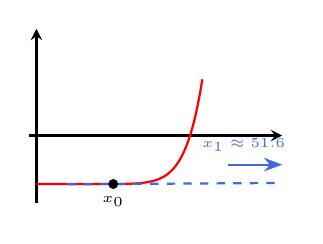
\begin{tikzpicture}
\begin{axis}[miniplot, width=4.8cm, height=3.8cm, xmin=-0.05, xmax=1.6, ymin=-1.4, ymax=2.2, clip=false]
  \addplot[red, domain=0:1.08, samples=150] {x^10-1};
  \addplot[accent, dashed, domain=0.2:1.6] {-0.99902+0.01953*(x-0.5)};
  \fill (axis cs:0.5,-0.999) circle (1.8pt);
  \node[font=\tiny, below] at (axis cs:0.5,-1.05) {$x_0$};
  \draw[-{Stealth}, accent] (axis cs:1.25,-0.6) -- (axis cs:1.6,-0.6);
  \node[accent, font=\tiny, above] at (axis cs:1.35,-0.55) {$x_1 \approx 51.6$};
\end{axis}
\end{tikzpicture}\\[3pt]
\textbf{Flat tangent: overshoot}\\[2pt]
\scriptsize $f(x) = x^{10}-1$, $x_0 = 0.5$: $f'(x_0) \approx 0.02$, so the step is huge. It then takes \textbf{42 steps} to crawl back. If $f'(x_n) = 0$ exactly, the step is undefined.
\end{column}
\begin{column}{0.32\textwidth}
\centering
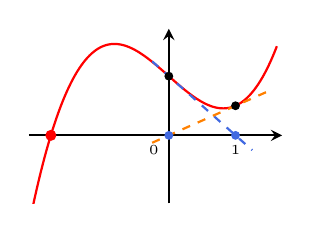
\begin{tikzpicture}
\begin{axis}[miniplot, width=4.8cm, height=3.8cm, xmin=-2.1, xmax=1.7, ymin=-2.3, ymax=3.6]
  \addplot[red, domain=-2.05:1.62] {x^3-2*x+2};
  \addplot[accent, dashed, domain=-0.25:1.25] {2-2*x};
  \addplot[orange, dashed, domain=-0.25:1.5] {x};
  \fill (axis cs:0,2) circle (1.6pt);
  \fill (axis cs:1,1) circle (1.6pt);
  \fill[accent] (axis cs:0,0) circle (1.6pt);
  \fill[accent] (axis cs:1,0) circle (1.6pt);
  \node[font=\tiny, below left] at (axis cs:0,0) {$0$};
  \node[font=\tiny, below] at (axis cs:1,0) {$1$};
  \fill[red] (axis cs:-1.769,0) circle (2pt);
\end{axis}
\end{tikzpicture}\\[3pt]
\textbf{Cycling}\\[2pt]
\scriptsize $f(x) = x^3 - 2x + 2$, $x_0 = 0$: the iterates go $0, 1, 0, 1, \ldots$ forever. The real root $r \approx -1.769$ is never reached.
\end{column}
\begin{column}{0.32\textwidth}
\centering
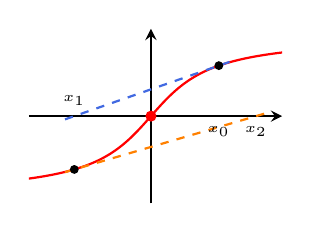
\begin{tikzpicture}
\begin{axis}[miniplot, width=4.8cm, height=3.8cm, xmin=-2.7, xmax=2.9, ymin=-1.7, ymax=1.7]
  \addplot[red, domain=-2.7:2.9] {rad(atan(x))};
  \addplot[accent, dashed, domain=-1.9:1.8] {0.98279+0.30769*(x-1.5)};
  \addplot[orange, dashed, domain=-1.9:2.5] {-1.03755+0.25840*(x+1.69408)};
  \fill (axis cs:1.5,0.98279) circle (1.6pt);
  \fill (axis cs:-1.69408,-1.03755) circle (1.6pt);
  \node[font=\tiny, below] at (axis cs:1.5,0) {$x_0$};
  \node[font=\tiny, above] at (axis cs:-1.69408,0) {$x_1$};
  \node[font=\tiny, below] at (axis cs:2.32,0) {$x_2$};
  \fill[red] (axis cs:0,0) circle (2pt);
\end{axis}
\end{tikzpicture}\\[3pt]
\textbf{Divergence}\\[2pt]
\scriptsize $f(x) = \arctan x$, root $0$. From $x_0 = 1.5$: $\;-1.69,\ 2.32,\ -5.11,\ 32.3, \ldots$ Each step overshoots more. From $x_0 = 1.3$ it converges.
\end{column}
\end{columns}
\end{frame}

\begin{frame}{Multiple roots: Newton slows down to linear}
\begin{columns}[T]
\begin{column}{0.5\textwidth}
\small
$f(x) = (x-1)^2$ has a \textbf{double root}: $f(1) = f'(1) = 0$. Newton still converges, but slowly ($x_0 = 2$):

\vspace{0.1cm}
\centering
\footnotesize
\begin{tabular}{rcc}
\toprule
$n$ & $x_n$ & $|x_n - 1|$ \\
\midrule
0 & 2 & 1 \\
1 & 1.5 & 0.5 \\
2 & 1.25 & 0.25 \\
3 & 1.125 & 0.125 \\
$\vdots$ & & $\vdots$ \\
\bottomrule
\end{tabular}\\[3pt]
\raggedright
\scriptsize Linear with $\rho = \tfrac12$: no better than bisection. Here $f'(r) = 0$, so the theorem does not apply.
\end{column}
\begin{column}{0.47\textwidth}
\begin{block}{Root of multiplicity $m$}
\footnotesize If $f(x) = (x - r)^m\,h(x)$ with $h(r) \neq 0$, then
\[
e_{n+1} \approx \Big(1 - \frac1m\Big)\,e_n .
\]
Linear, with $\rho = 1 - \tfrac1m$: worse for higher $m$.
\end{block}
\begin{exampleblock}{Fix: modified Newton}
\footnotesize If $m$ is known,
\[
x_{n+1} = x_n - m\,\frac{f(x_n)}{f'(x_n)}
\]
is quadratic again ($(x-1)^2$, $m = 2$: exact in one step).
\end{exampleblock}
\scriptsize Symptom: the step only halves each iteration.
\end{column}
\end{columns}
\end{frame}

% ============================================================
\section{Safeguarded Newton}
% ============================================================

\begin{frame}[fragile]{Best of both: Newton with a bracket}
\begin{columns}[T]
\begin{column}{0.56\textwidth}
\begin{lstlisting}[basicstyle=\ttfamily\scriptsize]
def safe_newton(f, df, a, b, tol=1e-10, maxit=100):
    fa = f(a)
    if np.sign(fa) == np.sign(f(b)):
        raise ValueError("not a bracket")
    x = a + (b - a)/2
    for n in range(maxit):
        fx, dfx = f(x), df(x)
        if np.sign(fx) == np.sign(fa):
            a, fa = x, fx          # root in [x, b]
        else:
            b = x                  # root in [a, x]
        if dfx != 0:
            xnew = x - fx/dfx      # try Newton
        if dfx == 0 or not (a <= xnew <= b):
            xnew = a + (b - a)/2   # fall back
        if abs(xnew - x) < tol:
            return xnew
        x = xnew
    return x
\end{lstlisting}
\end{column}
\begin{column}{0.41\textwidth}
\begin{block}{Rule}
\footnotesize Keep a bracket $[a,b]$ all the time. Take the Newton step if it lands \textbf{inside} the bracket; otherwise take a \textbf{bisection} step.
\end{block}
\begin{itemize}\scriptsize
  \item \textbf{Guaranteed} to converge, like bisection.
  \item Near the root, Newton steps land inside: \textbf{quadratic}.
\end{itemize}
\centering
\scriptsize
\setlength{\tabcolsep}{3pt}
\begin{tabular}{lr}
\toprule
$x^{10} - 1$ on $[0, 1.3]$ & steps to $10^{-6}$ \\
\midrule
bisection & 20 \\
false position & 61 \\
Illinois & 13 \\
Newton, $x_0 = 0.65$ & 21 \\
safeguarded Newton & \cbox{green!15}{4} \\
\bottomrule
\end{tabular}\\[2pt]
\raggedright
\tiny Plain Newton from the midpoint jumps to $x_1 \approx 5.4$. The safeguard bisects once, then 3 Newton steps.
\end{column}
\end{columns}
\end{frame}

% ============================================================
\section{Newton without derivatives}
% ============================================================

\begin{frame}{Newton without derivatives: approximate the slope}
\begin{columns}[T]
\begin{column}{0.52\textwidth}
\small
Newton's idea only needs \textbf{a slope} at $x_n$. If $f'$ is unknown or expensive, approximate it.
\begin{block}{Option 1: finite-difference Newton}
\footnotesize
\[
f'(x_n) \approx \frac{f(x_n + h) - f(x_n)}{h}
\]
with $h \approx \sqrt{\varepsilon_{\text{mach}}}\,|x_n| \approx 10^{-8}|x_n|$. Still \textbf{2 evaluations} per step.
\end{block}
\begin{exampleblock}{Option 2: reuse the previous point}
\footnotesize
We already know $f(x_{n-1})$. Use it, for \textbf{free}:
\[
f'(x_n) \approx \frac{f(x_n) - f(x_{n-1})}{x_n - x_{n-1}}.
\]
This is the \textbf{secant method}.
\end{exampleblock}
\end{column}
\begin{column}{0.45\textwidth}
\centering
\footnotesize
Finite-difference Newton, $x^2 - 2$, $x_0 = 1$:\\[3pt]
\setlength{\tabcolsep}{4pt}
\begin{tabular}{rcc}
\toprule
$n$ & $h = 10^{-8}$ & $h = 10^{-3}$ \\
\midrule
1 & $8.6\times10^{-2}$ & $8.6\times10^{-2}$ \\
2 & $2.5\times10^{-3}$ & $2.5\times10^{-3}$ \\
3 & $2.1\times10^{-6}$ & $3.0\times10^{-6}$ \\
4 & $1.6\times10^{-12}$ & $1.1\times10^{-9}$ \\
5 & $2.2\times10^{-16}$ & $3.8\times10^{-13}$ \\
\bottomrule
\end{tabular}\\[4pt]
\raggedright
\scriptsize
\begin{itemize}
  \item $h = 10^{-8}$: same errors as exact Newton.
  \item $h = 10^{-3}$: slope error $\approx h$, so convergence drops below quadratic.
  \item $h$ too small ($\ll 10^{-8}$): rounding in $f(x_n+h) - f(x_n)$ ruins the slope.
\end{itemize}
\end{column}
\end{columns}
\end{frame}

\begin{frame}{The secant method}
\begin{columns}[c]
\begin{column}{0.5\textwidth}
\small
Put the secant slope into Newton's formula:
\[
\cbox{accent!12}{x_{n+1} = x_n - f(x_n)\,\frac{x_n - x_{n-1}}{f(x_n) - f(x_{n-1})}}
\]
\begin{itemize}\footnotesize
  \item Needs \textbf{two} starting points $x_0, x_1$, no bracket, no $f'$.
  \item Same formula as false position, but always keeps the \textbf{two newest} points: no endpoint gets stuck, and no guarantee.
  \item Order $p = \frac{1+\sqrt5}{2} \approx 1.618$ with \textbf{1 evaluation} per step.
\end{itemize}
\vspace{0.05cm}
\centering
\scriptsize
\setlength{\tabcolsep}{3pt}
\begin{tabular}{lcc}
\toprule
$\sqrt2$, tol $= 10^{-6}$ & steps & $f$/$f'$ evaluations \\
\midrule
Newton, $x_0 = 1$ & 4 & 8 \\
secant, $x_0 = 1$, $x_1 = 2$ & 5 & \cbox{green!15}{7} \\
\bottomrule
\end{tabular}
\end{column}
\begin{column}{0.47\textwidth}
\centering
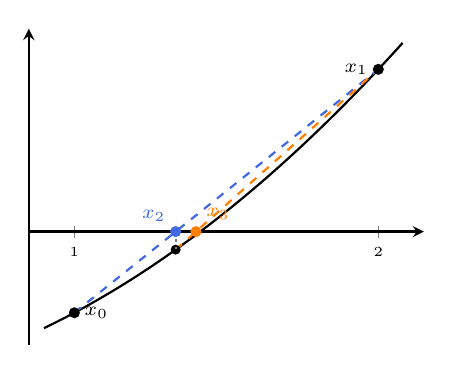
\begin{tikzpicture}
\begin{axis}[width=6.6cm, height=5.6cm, axis lines=middle, xmin=0.85, xmax=2.15, ymin=-1.4, ymax=2.5,
  xtick={1,2}, ytick=\empty, samples=80, thick, tick label style={font=\tiny}, clip=false]
  \addplot[black, domain=0.9:2.08] {x^2-2};
  \addplot[accent, dashed, domain=1:2] {3*x-4};
  \addplot[orange, dashed, domain=1.3333:2] {2+3.3333*(x-2)};
  \fill (axis cs:1,-1) circle (2pt) node[right, font=\scriptsize] {$x_0$};
  \fill (axis cs:2,2) circle (2pt) node[left, font=\scriptsize] {$x_1$};
  \fill (axis cs:1.3333,-0.2222) circle (1.8pt);
  \draw[gray, dotted, thick] (axis cs:1.3333,0) -- (axis cs:1.3333,-0.2222);
  \fill[accent] (axis cs:1.3333,0) circle (2pt);
  \node[accent, font=\scriptsize, above left] at (axis cs:1.3333,0) {$x_2$};
  \fill[orange] (axis cs:1.4,0) circle (2pt);
  \node[orange, font=\scriptsize, above right] at (axis cs:1.4,0.02) {$x_3$};
\end{axis}
\end{tikzpicture}\\[2pt]
\scriptsize Errors: $10^{-2} \to 10^{-4} \to 10^{-6} \to 10^{-10} \to 10^{-16}$.\\ Exponents grow by $\approx 1.6\times$ per step (Newton: $2\times$).
\end{column}
\end{columns}
\end{frame}

% ============================================================
\section{Stopping and cost}
% ============================================================

\begin{frame}{When do we stop?}
\begin{columns}[T]
\begin{column}{0.52\textwidth}
\small
No bracket, so no guaranteed error bound. But quadratic convergence makes the \textbf{step size} a very good error estimate:
\[
x_{n+1} - x_n = e_{n+1} - e_n \approx -e_n
\quad\text{since } |e_{n+1}| \ll |e_n|.
\]
So $|x_{n+1} - x_n| \approx |e_n|$, and $x_{n+1}$ is \textbf{even more accurate} than that.
\end{column}
\begin{column}{0.45\textwidth}
\begin{exampleblock}{Practical recipe}
\small
\begin{itemize}
  \item Plot $f$; pick $x_0$ near the root (or a bracket).
  \item Stop when $|x_{n+1} - x_n| < \text{tol}\cdot|x_{n+1}|$.
  \item Cap with \texttt{maxit}; \textbf{raise} if reached.
\end{itemize}
\end{exampleblock}
\begin{alertblock}{Floating point floor}
\scriptsize Once $|e_n| \approx 10^{-16}|r|$, iterates only jiggle by rounding. Don't ask for more.
\end{alertblock}
\end{column}
\end{columns}
\end{frame}

\begin{frame}{Comparison: bracketing vs.\ Newton vs.\ secant}
\begin{columns}[c]
\begin{column}{0.58\textwidth}
\centering
\scriptsize
\setlength{\tabcolsep}{2.5pt}
\begin{tabular}{lcccc}
\toprule
 & bisection & false pos. & Newton & secant \\
\midrule
needs & bracket & bracket & $x_0$, $f'$ & $x_0$, $x_1$ \\
always converges & yes & yes & \textbf{no} & \textbf{no} \\
order $p$ & 1 & 1 & \textbf{2} & 1.618 \\
evaluations per step & 1 & 1 & 2 & 1 \\
order per evaluation & 1 & 1 & 1.41 & \textbf{1.618} \\
error bound in advance & yes & no & no & no \\
double roots & no & no & linear & linear \\
\bottomrule
\end{tabular}
\end{column}
\begin{column}{0.39\textwidth}
\begin{block}{Counting work fairly}
\footnotesize Newton does 2 evaluations per step, so per \textbf{evaluation} its order is $2^{1/2} \approx 1.41$. The secant method ($1.618$) is the most efficient per evaluation. Newton wins when $f'$ is cheap: it often shares most of its work with $f$.
\end{block}
\begin{alertblock}{Rule of thumb}
\footnotesize Reliability from brackets, speed from Newton: in practice, combine them.
\end{alertblock}
\end{column}
\end{columns}
\end{frame}

% ============================================================
\section{Summary}
% ============================================================

\begin{frame}{Summary}
\begin{columns}[T]
\begin{column}{0.24\textwidth}
\begin{block}{Newton's method}
\scriptsize
\begin{itemize}
  \item $x_{n+1} = x_n - \frac{f(x_n)}{f'(x_n)}$
  \item zero of the tangent line
  \item needs $x_0$ and $f'$, no bracket
\end{itemize}
\end{block}
\end{column}
\begin{column}{0.24\textwidth}
\begin{block}{Convergence}
\scriptsize
\begin{itemize}
  \item $e_{n+1} \approx \frac{f''(r)}{2f'(r)}\, e_n^2$
  \item quadratic: digits double
  \item only if $x_0$ is close and $f'(r) \ne 0$
  \item multiple root: linear
\end{itemize}
\end{block}
\end{column}
\begin{column}{0.24\textwidth}
\begin{block}{No derivative}
\scriptsize
\begin{itemize}
  \item finite differences, $h \approx 10^{-8}|x|$
  \item secant: slope from the last two points
  \item order $1.618$, 1 evaluation per step
\end{itemize}
\end{block}
\end{column}
\begin{column}{0.24\textwidth}
\begin{block}{In practice}
\scriptsize
\begin{itemize}
  \item can overshoot, cycle, diverge
  \item safeguard with a bracket
  \item stop on step size, cap \texttt{maxit}
  \item raise an error if it fails
\end{itemize}
\end{block}
\end{column}
\end{columns}
\vspace{0.4cm}
\centering
\small Newton's idea: fastest when it works, so start it close or protect it with a bracket.\\[3pt]
\scriptsize Next session: root finding with \texttt{scipy.optimize} (\texttt{newton}, \texttt{brentq}, \texttt{root\_scalar}).
\end{frame}

\end{document}
